\section{Finding vulnerabilities}\label{theory_finding_vulns}
Armed with the information provided by the reaching definitions analysis we should be able to find vulnerabilities in applications.
The vulnerabilities mentioned in \cref{security_vulnerabilities} all have in common that one expression introduces user input into the program, and a later expression executes this input.
The structure of such application is outlined on \cref{vulnerabilities_unsanitised}.
Untrusted user input is denoted as a \emph{source}, while a piece of sensitive code is denoted as a \emph{sink}.

Using the reaching definitions analysis it is possible to determine if the data obtained at the source will reach the sink, by examining the constraints provided by the analysis.
If the source is contained in the set of contraints of the sink, we can regard is a potential security vulnerability.

Such a vulnerability can potentially be harmless because of processing on the path towards the sink.
A function that takes some untrusted input and returns a harmless version will be denoted as a \emph{sanitiser}.
\Cref{vulnerabilities_sanitised} shows the outline of an application with a sanitiser.
The flow of such a program makes it impossible to guarantee that the application is safe, but reporting it to the developer may ease the process of securing the application.



\begin{figure}
  \begin{subfigure}[b]{0.5\textwidth}
    \centering
    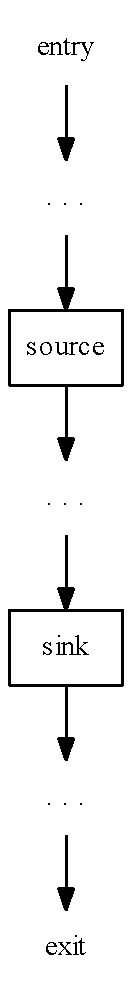
\includegraphics[scale=0.8]{figures/dot_files/unsanitised.pdf}
    \caption{A vulnerable application}\label{vulnerabilities_unsanitised}
  \end{subfigure}
  ~
  \begin{subfigure}[b]{0.5\textwidth}
    \centering
    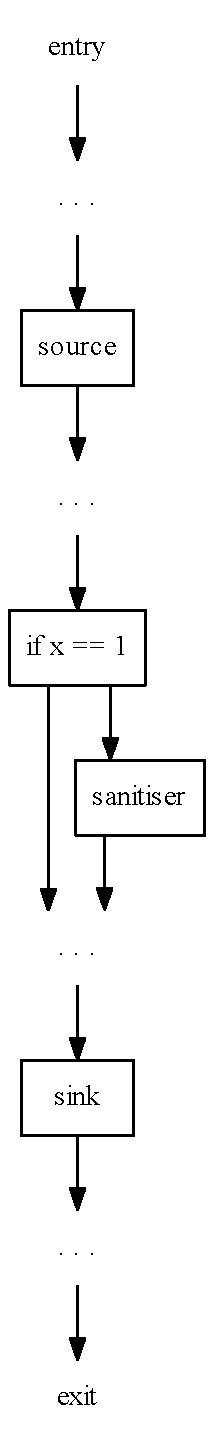
\includegraphics[scale=0.8]{figures/dot_files/sanitised_with_flow.pdf}
    \caption{A sanitiser eliminating the vulnerability}
    \label{vulnerabilities_sanitised}
  \end{subfigure}
  
  \caption{Control Flow Graphs for appliations with potential vulnerabilities}
\end{figure}
\todo{draft, vi skal nok overveje denne sektion igen når vi har alle detaljer omkring taint, propagation og sanitiser handling på plads}
